% =====================================================================
%  Figure captions for
%  "Carry the Uncertainty, Not the Knowledge:
%   A Tandem Knapsack--Cascade Calculus ..."
%
%  Seven validation panels, one per theorem. Each panel is a row of four
%  data charts on a white background with at least one 3-D chart. Every
%  number below is measured by validation/run_validation.py and the panel
%  generator figures/make_panels.py under the fixed seed 42.
%
%  \input this file inside the document body, or copy the individual
%  figure* blocks where each panel should sit.
% =====================================================================

\begin{figure*}[!htbp]
    \centering
    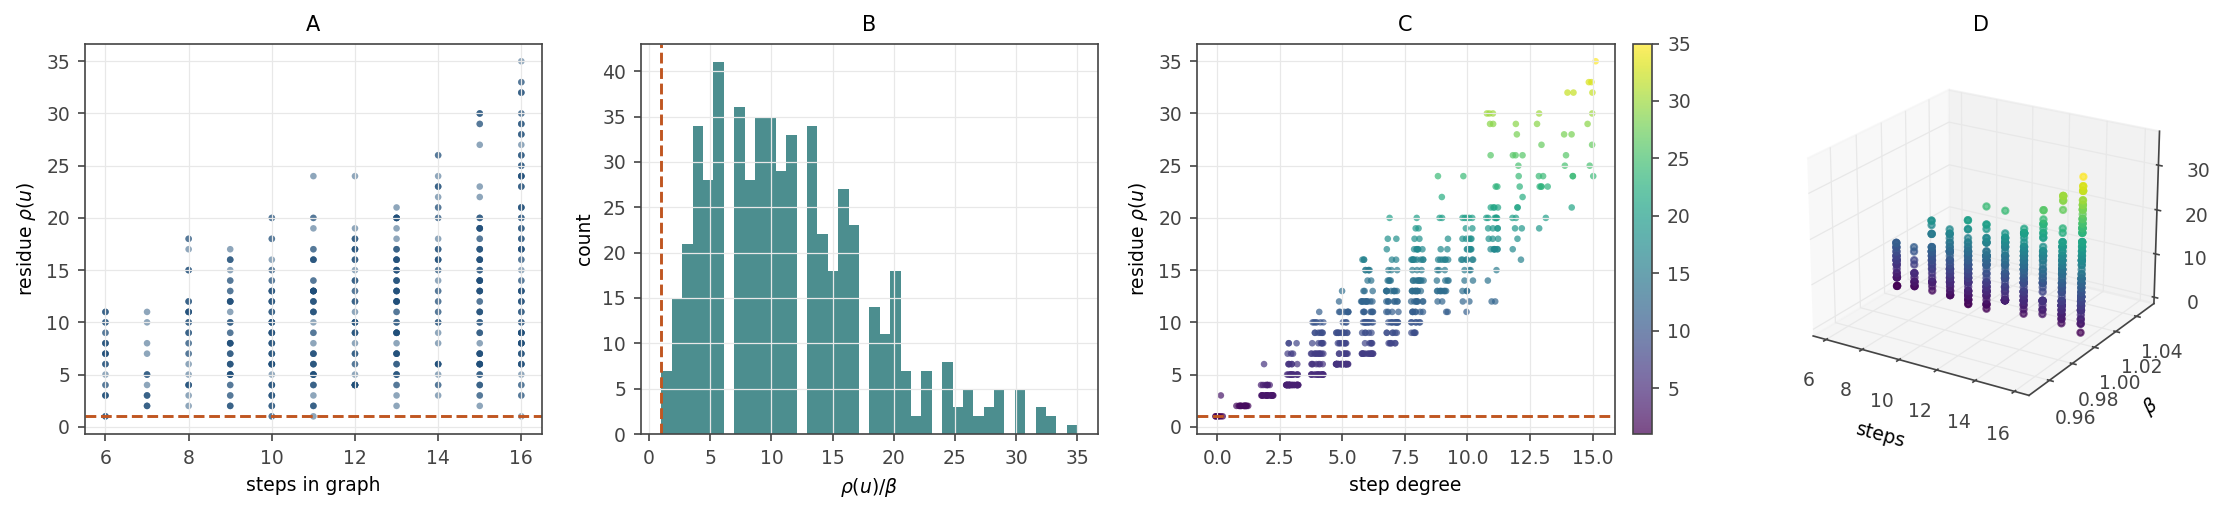
\includegraphics[width=\textwidth]{figures/panel1_floor.png}
    \caption{\textbf{The Floor Is Positive and No Residue Crosses It.}
    (\textbf{A})~Residue $\rho(u)$ of every step against the number of steps in
    its graph, for $562$ steps drawn from $50$ random context graphs. The orange
    dashed line marks the floor $\beta$; every point lies on or above it, and the
    residue ceiling rises with graph size to a maximum of $35$. Empirical content
    of the Floor Theorem~\ref{thm:floor}: telling a step apart from the medium
    costs at least $\beta > 0$.
    (\textbf{B})~Distribution of the normalised residue $\rho(u)/\beta$ across the
    same $562$ steps, supported entirely at and above $1$ with a minimum of
    exactly $1.0$ and a long right tail to $35.0$. No step falls below the floor
    ($0$ violations), and the mass concentrated near $1$ is the population of
    steps individuated by a single shared-term edge, the cheapest genuine
    separation.
    (\textbf{C})~Residue against step degree over shared-term edges, colour-mapped
    by $\rho(u)/\beta$ (viridis). The floor line (orange dashed) bounds the cloud
    below at every degree; residue grows with the number of distinctions a step
    shares, but never dips beneath $\beta$. This isolates the driver of a step's
    separation cost --- how many other steps it is entangled with --- while the
    lower bound remains the floor.
    (\textbf{D})~Three-dimensional scatter of $(\text{steps},\,\beta,\,\rho(u))$
    with the floor plane $\rho = \beta$ (orange, semi-transparent), viewing angle
    elevation $22^{\circ}$, azimuth $-58^{\circ}$. The entire point cloud sits on
    or above the plane at every graph size, the geometric realisation of
    Corollary~\ref{cor:trace}: the floor is the trace the non-completable medium
    casts on each finite part, uniform across the size of the model.}
    \label{fig:floor}
\end{figure*}

\begin{figure*}[!htbp]
    \centering
    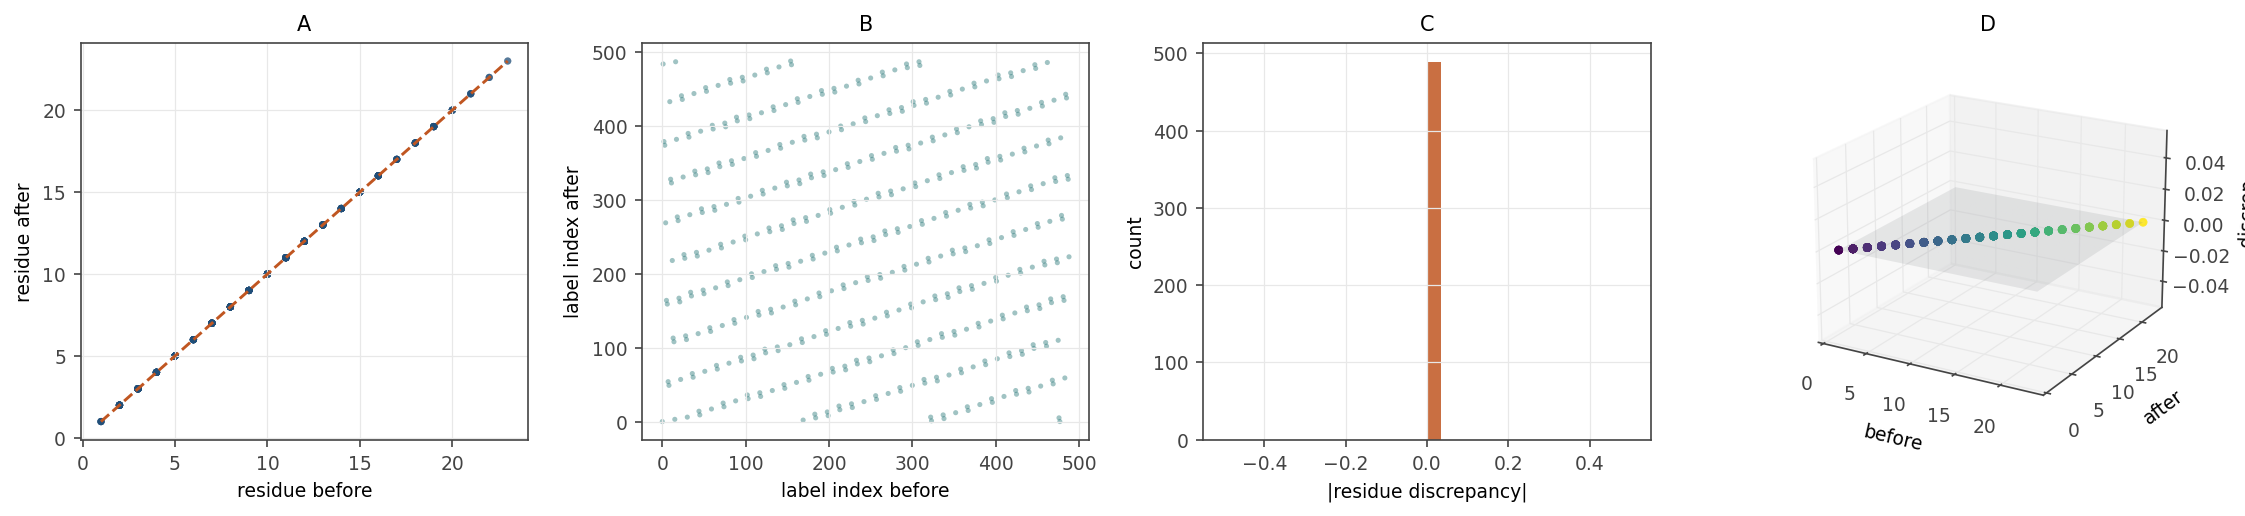
\includegraphics[width=\textwidth]{figures/panel2_invariance.png}
    \caption{\textbf{Residue Is Conserved Under Re-encoding; Labels Are Not.}
    (\textbf{A})~Residue after a random re-encoding (a weighted relabelling of the
    steps) against residue before, for every step of $50$ random graphs. All
    points lie exactly on the identity diagonal (orange dashed): the re-encoding
    preserves each step's residue to machine precision. Empirical content of the
    Invariance Theorem~\ref{thm:invariant}.
    (\textbf{B})~The corresponding label indices after against before, scattered
    off the diagonal across the whole square. The datum the re-encoding moves is
    exactly the label --- the relabellable surface --- while (A) shows the datum
    it fixes is the residue. Together the two panels separate the invariant from
    the surface on the same instances.
    (\textbf{C})~Distribution of the per-step residue discrepancy
    $\lvert\rho_{\text{before}} - \rho_{\text{after}}\rvert$, a single bar at zero:
    the maximum discrepancy over all steps is $0$. The invariant is preserved not
    approximately but exactly, because a weighted isomorphism carries each
    step--medium cut to an equal-weight cut.
    (\textbf{D})~Three-dimensional scatter of
    $(\rho_{\text{before}},\,\rho_{\text{after}},\,\text{discrepancy})$ with the
    zero-discrepancy plane (grey), elevation $20^{\circ}$, azimuth $-60^{\circ}$.
    The cloud lies flat on the plane along the before-equals-after ridge,
    exhibiting geometrically that the residue is the conserved object beneath the
    relabellable surface (Principle~\ref{prin:carry}).}
    \label{fig:invariance}
\end{figure*}

\begin{figure*}[!htbp]
    \centering
    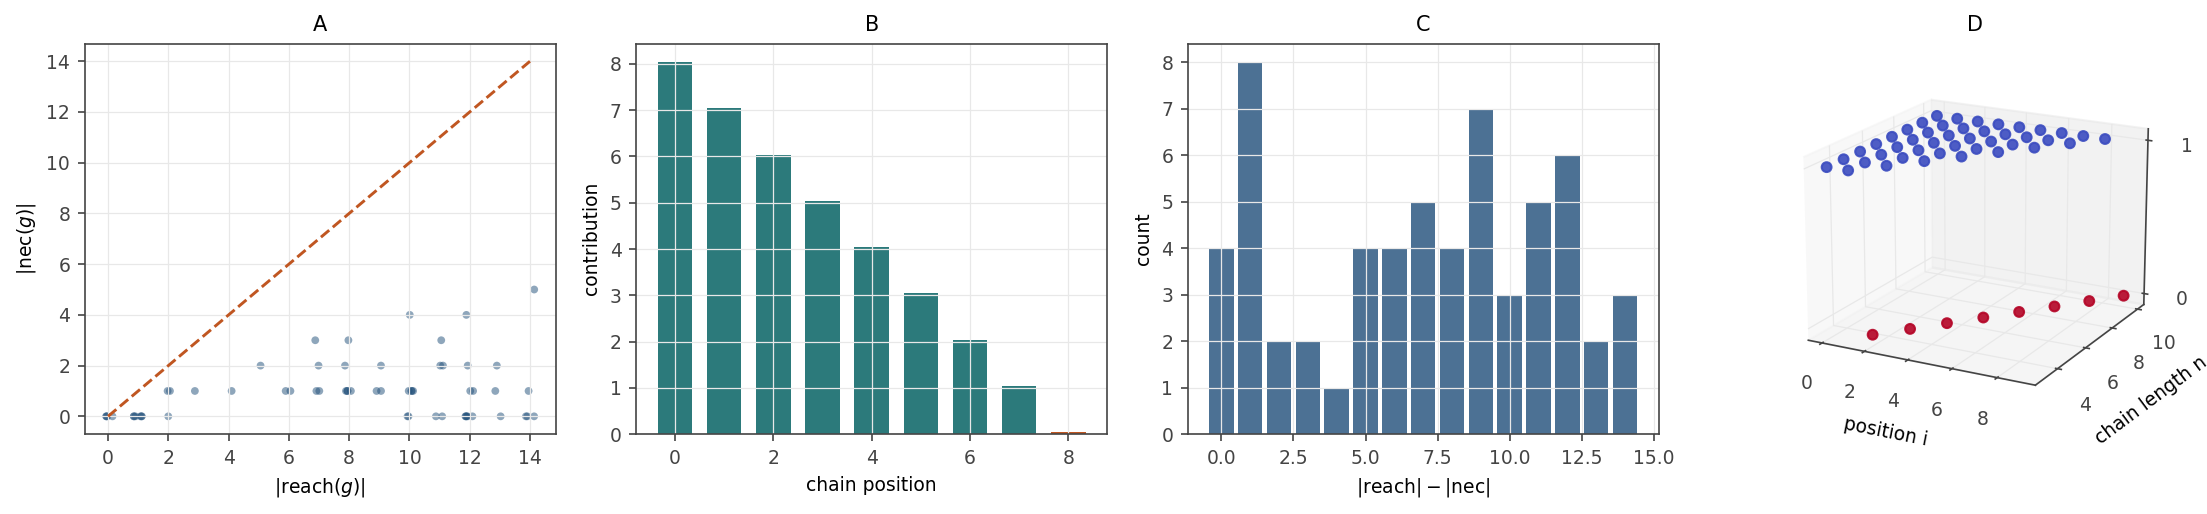
\includegraphics[width=\textwidth]{figures/panel3_necessity.png}
    \caption{\textbf{Necessity Is a Subset of Reachability, and Where They Split.}
    (\textbf{A})~Necessary-set size $\lvert\mathrm{nec}(g)\rvert$ against
    reachable-set size $\lvert\mathrm{reach}(g)\rvert$ over $60$ random goals
    (reachable size up to $14$). Every point lies on or below the identity
    diagonal (orange dashed): the inclusion $\mathrm{nec}(g) \subseteq
    \mathrm{reach}(g)$ held on all $60$ instances. This is the always-true half of
    the Necessity Theorem~\ref{thm:necessity} and Remark~\ref{rem:necessity-scope}.
    (\textbf{B})~Per-position contribution along a chain of length $9$ with the
    goal touching step $s_0$. The contribution decays monotonically from $8$ at
    $s_0$ to $1$ at $s_7$ and to exactly $0$ at the terminal leaf $s_8$ (orange
    bar): interior steps dominate their successors and are necessary, the leaf
    dominates nothing and is reachable yet redundant. This is the chain identity
    $\mathrm{nec}(g) = \mathrm{reach}(g) \setminus \{\text{terminal leaf}\}$ of
    Remark~\ref{rem:necessity-scope}.
    (\textbf{C})~Distribution of the gap $\lvert\mathrm{reach}\rvert -
    \lvert\mathrm{nec}\rvert$ over the $60$ random goals, ranging from $0$ up to
    $14$. A strictly positive gap is the over-retention a reachability-only carry
    would incur; its spread quantifies how much a $\mathrm{seek}$-only mechanism
    keeps beyond the load-bearing core.
    (\textbf{D})~Three-dimensional necessity map over
    $(\text{position } i,\,\text{chain length } n)$, colour by the necessity flag
    (red $=$ not necessary, blue $=$ necessary), elevation $18^{\circ}$, azimuth
    $-62^{\circ}$. The lower red band is the terminal leaf at every chain length
    --- never necessary --- and the upper blue band is the interior --- always
    necessary --- making the dominator characterisation of necessity visible
    across the whole family.}
    \label{fig:necessity}
\end{figure*}

\begin{figure*}[!htbp]
    \centering
    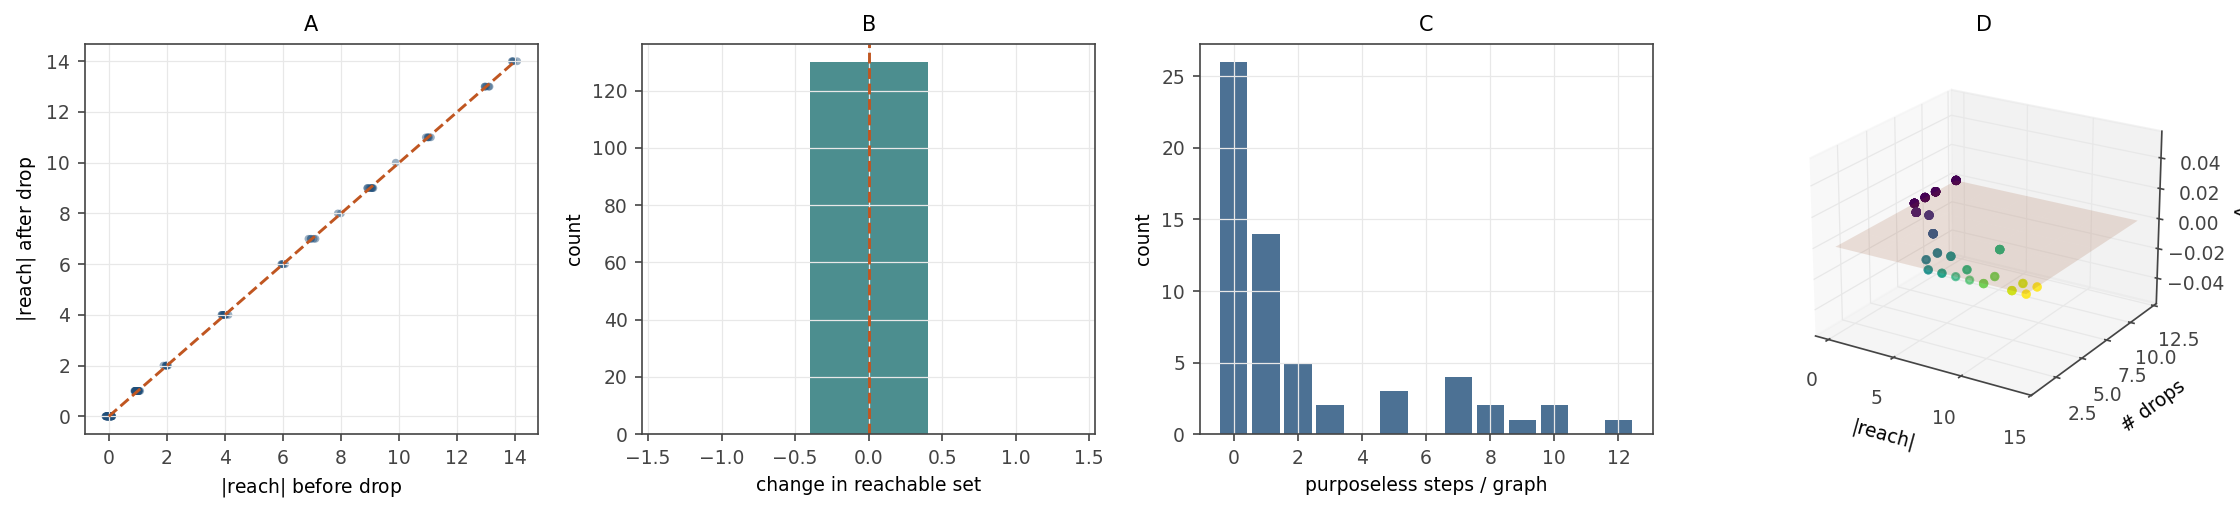
\includegraphics[width=\textwidth]{figures/panel4_freedrop.png}
    \caption{\textbf{Dropping a Purposeless Step Is Free.}
    (\textbf{A})~Reachable-set size after dropping an unreachable step against the
    size before, for every purposeless step of $60$ random graphs. All points lie
    exactly on the identity diagonal (orange dashed): removing a step the goal
    cannot reach leaves the goal's reachable resolution identical. Empirical
    content of the Free-Drop Theorem~\ref{thm:freedrop}.
    (\textbf{B})~Distribution of the change in the reachable set on each drop, a
    single bar at $0$ (orange reference line): $0$ violations. Forgetting a step
    the goal does not reach individuates nothing and deposits nothing on the
    carried invariant.
    (\textbf{C})~Distribution of the number of purposeless steps per graph, the
    population that is free to drop. That this count is routinely non-zero is why
    the free drop matters in practice: a real history carries steps disjoint from
    any given goal, and all of them are discardable at no cost to that goal.
    (\textbf{D})~Three-dimensional scatter of the change $\Delta$ over
    $(\lvert\mathrm{reach}\rvert,\,\text{number of drops})$ with the zero plane
    (orange), elevation $22^{\circ}$, azimuth $-58^{\circ}$. The cloud lies flat
    on $\Delta = 0$ regardless of how many purposeless steps are dropped or how
    large the reachable set is: the drop is free against the invariant uniformly.}
    \label{fig:freedrop}
\end{figure*}

\begin{figure*}[!htbp]
    \centering
    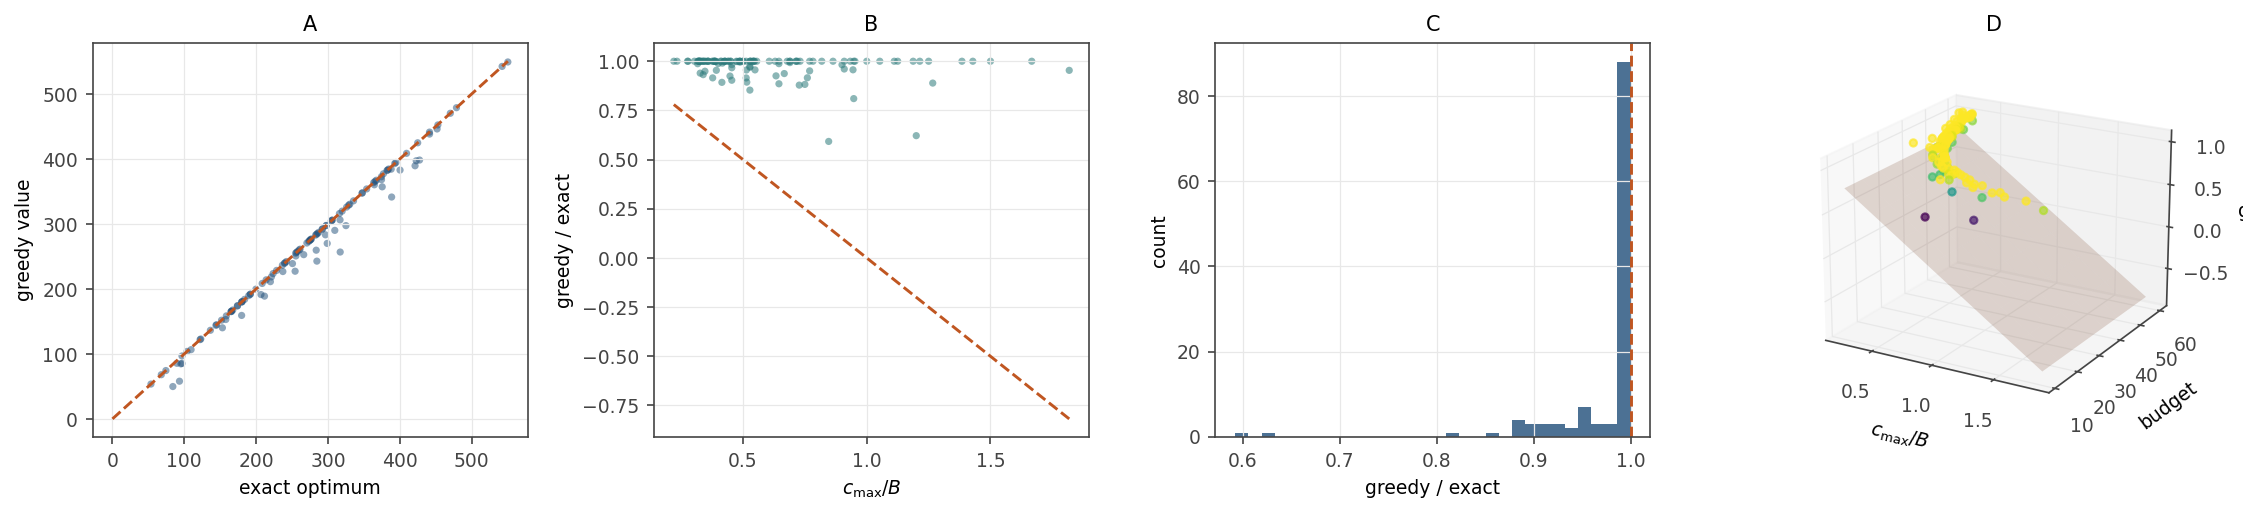
\includegraphics[width=\textwidth]{figures/panel5_knapsack.png}
    \caption{\textbf{The Value-Density Greedy Carry Is Near-Optimal.}
    (\textbf{A})~Greedy carry value against the exact dynamic-programming optimum
    over $120$ random carry instances. Every point lies on or below the identity
    diagonal (orange dashed) and the exact DP attained the optimum in all $120$
    trials: the greedy never exceeds, and the DP never misses, the optimum. This
    is the joint content of the Knapsack Theorem~\ref{thm:knapsack} and the
    Value-Density Greedy Theorem~\ref{thm:greedy}.
    (\textbf{B})~Greedy-to-exact ratio against $c_{\max}/B$, with the guaranteed
    lower bound $1 - c_{\max}/B$ drawn as the orange dashed line. All $120$ points
    lie on or above the bound (within-bound count $120/120$); the ratio degrades
    toward the bound only as a single item consumes a large fraction of the
    budget, exactly the boundary-item effect the theorem predicts.
    (\textbf{C})~Distribution of the greedy-to-exact ratio, concentrated near $1$
    with mean $0.975$ and minimum $0.592$. The worst realised relative gap is
    $0.408$, attained on a small tight-budget instance, and remains inside the
    $c_{\max}/B$ guarantee; the bulk of instances are near-exact.
    (\textbf{D})~Three-dimensional scatter of the greedy-to-exact ratio over
    $(c_{\max}/B,\,B)$ with the guarantee surface $z = 1 - c_{\max}/B$ (orange),
    colour by ratio (viridis), elevation $20^{\circ}$, azimuth $-60^{\circ}$. The
    point cloud sits on or above the surface throughout, the geometric statement
    that the greedy carry meets its worst-case guarantee across the whole
    budget/cost plane, ranking the carry by residue per token
    (Remark~\ref{rem:density}).}
    \label{fig:knapsack}
\end{figure*}

\begin{figure*}[!htbp]
    \centering
    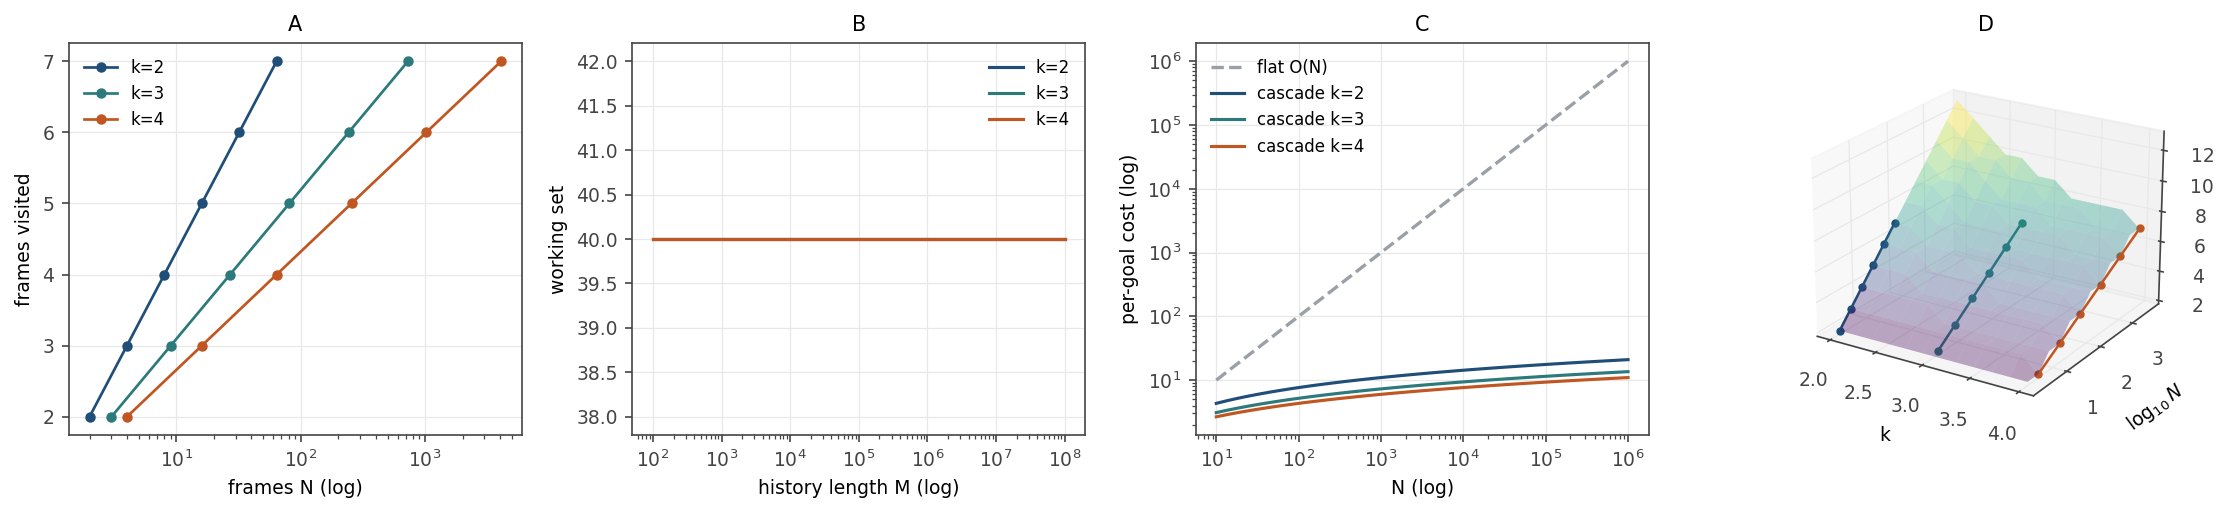
\includegraphics[width=\textwidth]{figures/panel6_cascade.png}
    \caption{\textbf{The Cascade Working Set Is Logarithmic and Independent of
    History Length.}
    (\textbf{A})~Frames visited to resolve a goal against the number of frames $N$
    (log axis) for branching factors $k \in \{2, 3, 4\}$. Each curve is the
    step function $\lceil\log_k N\rceil + 1$; at $N = 32, k = 2$ and at
    $N = 243, k = 3$ the descent visits exactly $6$ frames. Empirical content of
    the Cascade Theorem~\ref{thm:cascade}.
    (\textbf{B})~Resident working set against total history length $M$ (log axis,
    spanning $10^2$ to $10^8$) for the three branching factors, each a horizontal
    line. The working set is flat: it depends on the cascade depth and per-frame
    budget ($s = 8$) but carries no term in $M$, so history may grow without bound
    while the resident set stays constant.
    (\textbf{C})~Per-goal cost against $N$ (log--log axes): the flat carry's
    $\mathcal{O}(N)$ (grey dashed) against the cascade's $\log_k N$ for
    $k \in \{2, 3, 4\}$. The cascade curves lie far below the flat baseline and
    diverge from it as $N$ grows, the compounding per-goal saving of
    Remark~\ref{rem:cascade-cost}.
    (\textbf{D})~Three-dimensional surface of frames visited over
    $(k,\,\log_{10} N)$, the $\lceil\log_k N\rceil + 1$ law (viridis), with the
    per-branching-factor descent traces overlaid, elevation $22^{\circ}$, azimuth
    $-58^{\circ}$. The surface falls with increasing $k$ and rises only
    logarithmically with $N$, exhibiting that the working-set bound is
    $\mathcal{O}(s\log_k N)$ across the whole parameter plane.}
    \label{fig:cascade}
\end{figure*}

\begin{figure*}[!htbp]
    \centering
    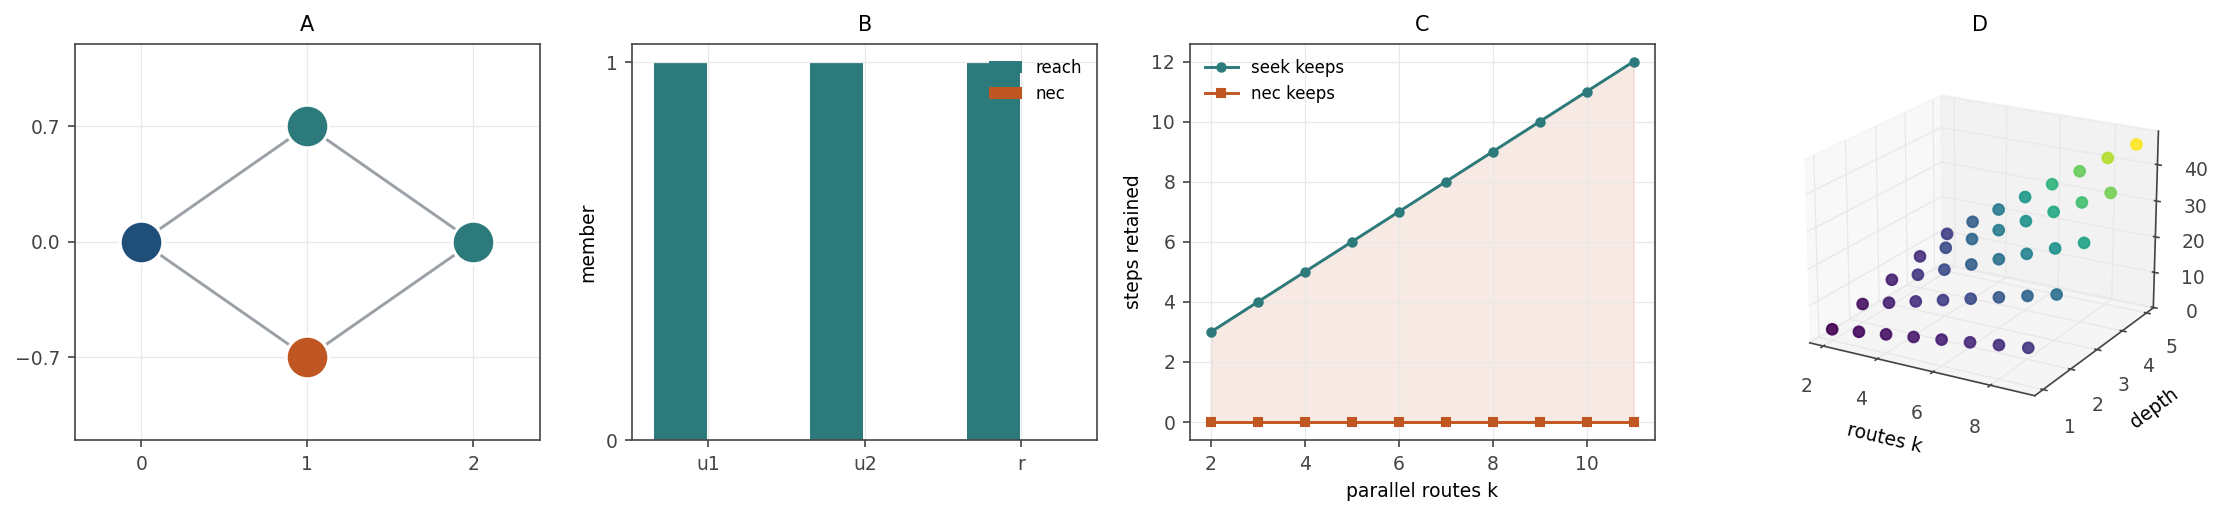
\includegraphics[width=\textwidth]{figures/panel7_separation.png}
    \caption{\textbf{Seek and Necessity Disagree: The Separation Witness.}
    (\textbf{A})~The diamond instance of the Separation Theorem~\ref{thm:separation}:
    the goal (left) reaches two steps $u_1, u_2$ (upper, lower), both feeding a
    common resolver $r$ (right). The redundant leg is drawn in orange. Both $u_1$
    and $u_2$ are reachable, but either alone suffices to reach $r$, so neither is
    individually load-bearing.
    (\textbf{B})~Membership of the three steps in $\mathrm{reach}(g)$ (teal) and
    $\mathrm{nec}(g)$ (orange). All three are reachable; the parallel legs are not
    necessary --- $\mathrm{reach}(g) = \{u_1, u_2, r\}$ while
    $\mathrm{nec}(g) = \varnothing$ for the pure parallel legs --- so
    $\mathrm{seek}$ and $\mathrm{nec}$ disagree on exactly the redundant steps.
    (\textbf{C})~Over a family of $k$ parallel routes to a shared resolver, the
    steps a $\mathrm{seek}$-only carry retains (teal, rising from $3$ at $k = 2$ to
    $12$ at $k = 11$) against the load-bearing steps $\mathrm{nec}$ retains
    (orange, flat near zero). The shaded region between them is the over-retention
    a reachability-only carry incurs; it grows linearly in the number of parallel
    routes, the practical cost of running $\mathrm{seek}$ without the necessity
    operator (Corollary~\ref{cor:no-single}).
    (\textbf{D})~Three-dimensional scatter of the $\mathrm{seek} - \mathrm{nec}$
    over-retention gap over $(\text{parallel routes } k,\,\text{route depth})$,
    colour by gap (viridis), elevation $20^{\circ}$, azimuth $-60^{\circ}$. The
    gap rises with both the number of parallel routes and their depth, exhibiting
    that the two operators diverge more sharply as redundancy compounds --- the
    structural reason the minimal correct architecture is the tandem
    $\mathrm{nec} \circ \mathrm{seek}$, not either operator alone.}
    \label{fig:separation}
\end{figure*}
